%%%%%%%%%%%%%%%%%%%%%%%%%%%%%%%%%%%%%%%%%%%%%%%%%%%%%%%%%%%%%%%%%%%%%%%%%%%%%%%%
%2345678901234567890123456789012345678901234567890123456789012345678901234567890
%        1         2         3         4         5         6         7         8

\documentclass[letterpaper, 10 pt, conference]{ieeeconf}
  % use above line letter sized paper
%\documentclass[a4paper, 10pt, conference]{ieeeconf}
  % Use this line for a4 paper
\IEEEoverridecommandlockouts
  % Needed if you want to use the \thanks command
\overrideIEEEmargins
  % Needed to meet printer requirements.


% The following packages can be found on http:\\www.ctan.org
\usepackage{graphics} % for pdf, bitmapped graphics files
\usepackage{epsfig} % for postscript graphics files
%\usepackage{mathptmx} % assumes new font selection scheme installed
%\usepackage{times} % assumes new font selection scheme installed
\usepackage{amsmath} % assumes amsmath package installed
\usepackage{amssymb}  % assumes amsmath package installed
\usepackage{pstricks}
\usepackage[utf8]{inputenc}
\usepackage{color}


\newcommand{\TODO}[1]{\textcolor{green}{TODO : #1}} %pour liste ce qu'il reste à faire


\title{\LARGE \bf Feet and legs tracking using a smart rollator
 }

\author{
C. Joly, C. Dune,  P. Gorce, P. Rives
\thanks{C.Joly, C. Dune and P. Gorce are with
Handibio, EA4322 Université du Sud- Toulon Var, France. 
}
\thanks{P. Rives is
 with Lagadic team Inria Sophia Antipolis, France}
}

\begin{document}



\maketitle
\thispagestyle{empty}
\pagestyle{empty}


%%%%%%%%%%%%%%%%%%%%%%%%%%%%%%%%%%%%%%%%%%%%%%%%%%%%%%%%%%%%%%%%%%%%%%%%%%%%%%%%
\begin{abstract}
Clinical evaluation of frailty in the elderly is the first step to decide the degree of assistance they require. This evaluation is usually performed once and for all by filling standard forms with macro-information about standing and walking abilities. Advances in robotics make it possible to turn a standard assistance device into an augmented device. The existing tests could then be enriched by a new set of daily measured criteria derived from the daily use of standard assistance devices. In this paper we use a smart rollator, equipped with a kinect and odometers, for biomechanical gait analysis. This paper focuses on the method we develop to track the legs and feet position during walking. \TODO{a completer}
\end{abstract}
%%%%%%%%%%%%%%%%%%%%%%%%%%%%%%%%%%%%%%%%%%%%%%%%%%%%%%%%%%%%%%%%%%%%%%%%%%%%%%%%

\section{Introduction}

 Ageing in society is a worldwide issue that especially impacts northern countries. In France, due to the high care cost and to the limited number of rooms in care institution, the solution that has been chosen by care-givers, frail people and their family is to maintain elderly at home the longest and in the best conditions by giving them an\textit{ adapted assistance}.  \\

Clinical evaluation of frailty in the elderly is the first step to decide the degree of assistance they require. This evaluation is usually performed once and for all by filling standard forms with macro-information about standing and walking abilities, e.g. by measuring the time taken to walk $10m$. Advances in robotics make it possible to enhance a standard assistance device by adding sensors and actuators. The existing tests could  then be enriched by adding a new set of daily measured criteria derived from the daily use of standard assistance devices. This monitoring will allow to evaluate gait in ambulatory conditions, to measure the evolution of some pathologies, to refine diagnostics and to distinguish autonomy levels. The assistance device is not meant to be an alternative for clinical frailty observation but rather as a complementary tool that gives field information. The data acquired \textit{online} could also be used to control a robotics walker in order to prevent a fall. These new characteristics can extend the use of walkers to more diverse population. \\ 

The system used here is a \textit{smart rollator} equipped with sensors, for gait monitoring. The objective is to provide physicians with the features they are used to process to evaluate elderly frailty,  while maintaining a low cost  and ensuring a good ease of use and by embedding all the sensors on the walker without equipping the patient. And at best, the intelligent walker could deliver others relevant features that will enriched the existing feature set. 

The paper is organised as following : \TODO{Decrire l'organisation du papier}

\section{System description}

Depending on the degree of assistance they need, people are prescribed canes, crutches or walkers \cite{Joyce91}. The latter can be legged walker or wheeled walkers (rollators). A rollator can be defined as a frame with wheels. It has handles with brakes, and in some case a seat, a basket and a tray (see fig. \ref{fig:rollator}).

 \begin{figure}[h]
\centering
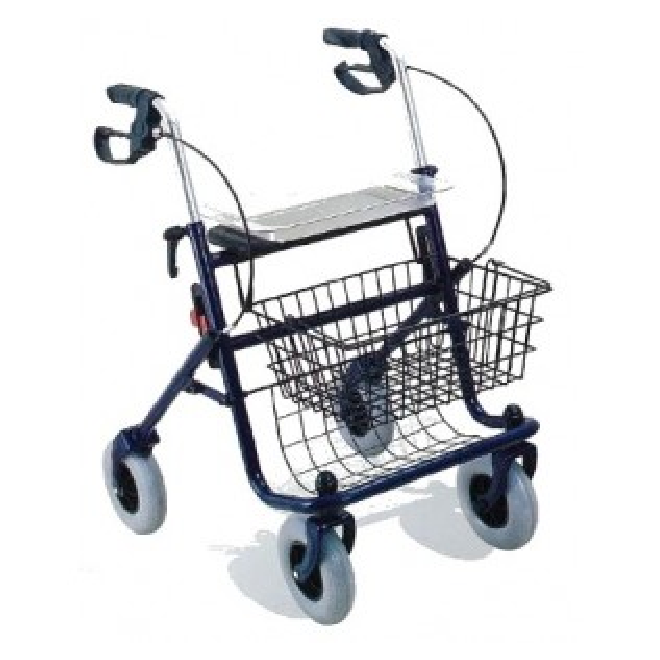
\includegraphics[width=0.45\columnwidth]{images/rollator.eps}
\caption{A 4 wheeled rollators}
\label{fig:rollator}
\end{figure}

Rollators induce a more natural gait pattern than standard four legged frames. They are designed for people that need less weight bearing~\cite{VanHook03}.

\subsection{Existing smart rollators}

Here is an overview of the the existing smart rollators, focusing on common wheeled walker that connects to a person at the hands. Smart walkers may be used to analyse either the environment or  the user's behaviour. Environmental data is dedicated to navigation purpose, such as obstacle avoidance~\cite{Spenko06}, wall following~\cite{Yu2003}, slope compensation~\cite{Hirata2007} or localisation~\cite{Kotani1996,MacNamara00}. Even though these functionalities are relevant for people autonomy, especially for the visually impaired, these functionalities are out of the scope of this paper that focuses on gait analyses. A thorough survey on assistance mobility device, focusing on smart walkers can be found in~\cite{Frizera08,Martins11}.\\

Some of the existing Smarts walkers aim at tracking the trajectories of gait features in order to monitor health. The great advantage of such systems is that the user stands at a roughly known position with regards to the walker. Body segment localisation is then made easier.

Walkers can be equipped with force-moment sensors mounted on the walker handles~\cite{Alwan07,Tung10}, or under the forearm~\cite{Frizera08,Frizera10b} to passively derive some gait characteristics. In both cases it is assumed that the force and moment recorded have cyclic changes reflecting the gait cycle and that these changes depend on basic gait features (cadence, stride time, gait phases).  The iWalker ~\cite{Tung10} quantifies loads exerted through the handles an frame and standards spatio-temporal parameters (such as speed and distance). In~\cite{Alwan07}, a direct comparison between motion capture and force-moment data was studied to detect significant pattern in the force signal. The lateral sway motion of the upper body reflects in peaks in vertical direction and in the corresponding forward moment signal. These peaks coincided with the heel initial contacts and. The forward propulsion force applied by the user is related to the toe-off event from the right and left toe. Finally, the stride (ie. duration of a gait cycle) can be computed from two heel contacts. In~\cite{Frizera10b}, a method based on Weighted Frequency Fourier Linear Combiner, is introduced for the same standards gait parameters extraction from force data.

Walker wheel motion measurement can also be used to estimated the user state~\cite{Spenko06,Merlet10b}. The Personal aid for mobility and monitoring project (PAMM)~\cite{Spenko06} developed health monitoring tools. The PAMM smart walker is an omnidirectional walker design for walking assistance with navigation and monitoring functionalities. Its sensors record user speed and compute the stride-to-stride variability, which have been shown to be an effective predictor of falls. A power spectrum analysis on PAMM's velocity allows to estimate user's stride length and frequency. Besides, the shape of the power spectrum is related to the gait symmetry. Indeed, for a symmetric gait, the energy is located at twice the stride frequency. However, the system can detect asymmetric gait as spectrum with energy located at the stride frequency and at higher frequency. An asymmetrical gait could be an indicator of a physical injury or a minor stroke.

Direct measurement of body segments may be obtained by using ultrasonics sensors or cameras \cite{Frizera08,Chee09}. A vector of ultrasonic sensors can be mounted on the walker to scan the space between the user and the walker and determine coordinate of each leg without adding any marker on the patient~\cite{Frizera08}. In ~\cite{Chee09}, a camera is mounted on the frame and observes markers on the toes. This marker based toe tracking algorithm allows to calculate step width and provide an accurate assessment of foot placement during rollator use.
  
The main issue when using that kind of device is that the accuracy of the leg localisation depends strongly on the clothes that the user wears. It is a drawback with regards to method based on odometers or force sensors. The method proposes in~\cite{Chee09} by-passes this point by adding markers on the toes. Yet it also by-passes our constraint not to equip the user in order to ensure acceptance and ease of use.

Extrinsic data can then be used to monitor the user's health or to control the walker in order to prevent a fall. The walker-user relative distance can be used to classify the states between a \textit{walking state}, a \textit{stopped state }and an \textit{emergency state} \cite{Hirata2006}. A laser range finder mounted on the walker acquired the position of the knee with regards to the walker frame. It is assumed that the position of the feet is at the vertical of the knee position, and fixing the human frame in the middle of the feet. User velocity is estimated from the walker velocity obtained by odometers. The\textit{ stopped state} occurs when both the walker and the human velocities are null. To distinguish the \textit{walking state} from the \textit{emergency state}, user-walker distance is used.  A normal distance distribution is computed to determine the  \textit{walking state} based on user data. The robot control tries to bring the user distance right to the mean of the  walking state distance distribution.

In~\cite{Hirata2008a} the RT-Walker is equipped with laser range finder and perform an estimation of the kinematics of a 7-link human model. The model is used to estimate the position of the user center of gravity (CoG) in 3D. A stable region is determined by analysing the distribution of the C.o.G. position for three subjects with different physiques who walked for 100 seconds with a walker. If the C.o.G is out of the region, the user may fall. The system then brakes enough to compensates for its lightweight and prevent the fall. Notice that the fall detection is restricted to the sagital plane.

In~\cite{Taghvaei10}, The RT Walker is equipped with vision sensor to classify the user state among four classes : sitting, standing, falling, and walking. The classifier is based on heuristic on the distance between user head, hands and shoulder. Basically, the vision algorithms are based on head tracking, and skin detection. Shoulder detection is performed by finding the higher points of a uniform color region under the head, which seems to lack robustness with regards to environment properties and user clothes.   

%Monitoring systems allow to estimate biomechanical features in ambulatory conditions, i.e. in uncontrolled conditions. Information about the walker itself (odometry, inertial parameters) or user-walker interaction seems more robust in these condition than laser data, video or distance sensors because they do not rely on environmental parameters such as user clothes and lightning condition. Yet, these sensors can provide useful and complementary information about user posture.

%Walking assistance based on user intend allows to control the direction of the walker. Fall prevention algorithm tend to draw the boundaries between "normal situations" and "risk of fall". Most of the time, the control strategy consists in braking to stop the system.
\subsection{Our smart rollator}


\TODO{Decrire ici notre system et les objectifs. Mettre une photo.}

In this paper, the system aims at tracking some specific parameters for biomechanical gait analysis, that were chosen in \cite{Dune2012}: 
\begin{itemize}
\item step length
\item step width
\item step frequency
\item feet orientation
\item heel trajectory
\item ankle angle trajectory
\end{itemize}

\section{Limb and feet tracking}



\subsection{Point cloud segmentation}

\subsection{Model fitting}

\subsection{Kalman filtering}

\section{Results}


\section{Conclusion}

\bibliographystyle{IEEEtran} 
\bibliography{biblio.bib}

% LIRMM D. Guiraud, P. Poignet, C. Azevedo Stimultation électrique fonctionnelle, étude de la posture
% P.B Wieber INRIA Grenoble

\end{document}





<!-- Local IspellDict: francais -->
